\documentclass[11pt,a4paper]{article}

% Packages modernes et professionnels
\usepackage[utf8]{inputenc}
\usepackage[english]{babel}
\usepackage[T1]{fontenc}
\usepackage{lmodern}
\usepackage{microtype}

% Mise en page moderne
\usepackage[margin=2.5cm]{geometry}
\usepackage{fancyhdr}
\usepackage{titlesec}
\usepackage{tocloft}

% Graphiques et images
\usepackage{graphicx}
\usepackage{float}
\usepackage{subcaption}
\usepackage{wrapfig}

% Tableaux professionnels
\usepackage{booktabs}
\usepackage{tabularx}
\usepackage{longtable}

% Mathématiques et code
\usepackage{amsmath}
\usepackage{amssymb}
\usepackage{listings}
\usepackage{xcolor}

% Liens et références
\usepackage{hyperref}
\usepackage{cleveref}
\usepackage{url}

% Design moderne des sections
\titleformat{\section}
  {\Large\bfseries\color{blue!80!black}}
  {\thesection}{1em}{}[\titlerule]

\titleformat{\subsection}
  {\large\bfseries\color{blue!60!black}}
  {\thesubsection}{1em}{}

% Configuration des liens
\hypersetup{
    colorlinks=true,
    linkcolor=blue!80!black,
    filecolor=magenta,
    urlcolor=blue!80!black,
    citecolor=blue!80!black,
    pdftitle={CNN Implementation Report},
    pdfauthor={Yassine Smaoui},
    pdfsubject={Artificial Intelligence - CNN Implementation},
    pdfkeywords={CNN, Deep Learning, TensorFlow, CIFAR-10, Image Classification}
}

% Configuration du code
\lstset{
    backgroundcolor=\color{gray!5},
    basicstyle=\ttfamily\small,
    keywordstyle=\color{blue!80!black}\bfseries,
    commentstyle=\color{green!60!black}\itshape,
    stringstyle=\color{red!70!black},
    numbers=left,
    numberstyle=\tiny\color{gray},
    stepnumber=1,
    numbersep=8pt,
    frame=leftline,
    frameround=tttt,
    framerule=0.5pt,
    rulecolor=\color{blue!30},
    breaklines=true,
    breakatwhitespace=true,
    tabsize=2,
    captionpos=b
}

% En-têtes et pieds de page
\pagestyle{fancy}
\fancyhf{}
\fancyhead[L]{\small\textsc{CNN Implementation Report}}
\fancyhead[R]{\small Yassine Smaoui}
\fancyfoot[C]{\thepage}
\renewcommand{\headrulewidth}{0.4pt}
\renewcommand{\footrulewidth}{0pt}

% Page de titre personnalisée
\makeatletter
\def\@maketitle{%
  \newpage
  \null
  \vspace{-2cm}
  \begin{center}%
    % Logo ou espace pour logo
    \vspace{2cm}
    
    % Informations institutionnelles
    {\large\textsc{Faculty of Polydisciplinary - Ouarzazate}\\[0.3cm]
    \textsc{Artificial Intelligence and Applications}\\[2cm]}
    
    % Titre principal
    {\Huge\bfseries\color{blue!80!black} CNN Implementation\\[0.5cm]
    \Large Deep Learning for Image Classification\\[2cm]}
    
    % Ligne de séparation
    \rule{12cm}{0.4pt}\\[1cm]
    
    % Informations du projet
    \begin{tabular}{ll}
      \textbf{Author:} & Yassine Smaoui \\[0.3cm]
      \textbf{Supervisor:} & M. Benaddy \\[0.3cm]
      \textbf{Program:} & Artificial Intelligence and Applications \\[0.3cm]
      \textbf{Institution:} & FP Ouarzazate \\[0.3cm]
      \textbf{Date:} & \today
    \end{tabular}\\[2cm]
    
    \rule{12cm}{0.4pt}\\[1cm]
    
    % Résumé court
    {\large\textit{A comprehensive implementation of Convolutional Neural Networks\\
    for image classification using TensorFlow and CIFAR-10 dataset}}
    
  \end{center}%
  \par
  \vfill
}
\makeatother

\begin{document}

\maketitle
\newpage

\tableofcontents
\newpage

\begin{abstract}
This report presents a comprehensive implementation of Convolutional Neural Networks (CNNs) for image classification tasks. The project focuses on building, training, and evaluating a CNN model using the CIFAR-10 dataset with TensorFlow/Keras framework. We explore various aspects of deep learning including data preprocessing, model architecture design, training optimization, and performance evaluation. The implementation demonstrates the effectiveness of CNNs for computer vision tasks, achieving significant accuracy on the multi-class image classification problem. Through detailed analysis and visualization, this work provides insights into the inner workings of convolutional neural networks and their practical applications in artificial intelligence.

\textbf{Keywords:} Convolutional Neural Networks, Deep Learning, Image Classification, TensorFlow, CIFAR-10, Computer Vision, Artificial Intelligence
\end{abstract}

\section{Introduction}

\subsection{Background and Motivation}

Convolutional Neural Networks (CNNs) represent one of the most significant breakthroughs in modern artificial intelligence, particularly in the field of computer vision. Since their introduction and popularization through architectures like LeNet, AlexNet, and more recently ResNet and EfficientNet, CNNs have revolutionized how machines perceive and understand visual information.

The motivation for this project stems from the fundamental importance of understanding CNN architectures in the context of artificial intelligence applications. Image classification serves as a cornerstone task that demonstrates the power of deep learning while providing practical insights into feature extraction, hierarchical learning, and pattern recognition.

\subsection{Objectives}

The primary objectives of this implementation are:

\begin{itemize}
    \item \textbf{Practical Implementation:} Build a complete CNN from scratch using modern deep learning frameworks
    \item \textbf{Architecture Understanding:} Explore the impact of different layers (convolution, pooling, normalization)
    \item \textbf{Training Optimization:} Implement best practices for model training including data augmentation and callbacks
    \item \textbf{Performance Analysis:} Conduct comprehensive evaluation using multiple metrics and visualization techniques
    \item \textbf{Methodology Documentation:} Provide detailed documentation of the entire workflow for reproducibility
\end{itemize}

\subsection{Dataset Selection}

For this implementation, we selected the CIFAR-10 dataset, which has become a standard benchmark in computer vision research. CIFAR-10 consists of 60,000 32×32 color images distributed across 10 mutually exclusive classes: airplane, automobile, bird, cat, deer, dog, frog, horse, ship, and truck. This dataset provides an ideal balance between complexity and computational requirements, making it suitable for educational purposes while remaining challenging enough to demonstrate real-world applications.

\section{Methodology}

\subsection{Technical Environment}

The implementation utilizes a modern Python-based machine learning stack:

\begin{itemize}
    \item \textbf{Framework:} TensorFlow 2.20.0 with Keras high-level API
    \item \textbf{Programming Language:} Python 3.12
    \item \textbf{Additional Libraries:} NumPy, Matplotlib, Scikit-learn, Seaborn
    \item \textbf{Development Environment:} Jupyter Notebook for interactive development and visualization
\end{itemize}

\subsection{Data Preprocessing and Augmentation}

Effective data preprocessing forms the foundation of successful deep learning implementations. Our preprocessing pipeline includes several critical steps:

\begin{figure}[H]
    \centering
    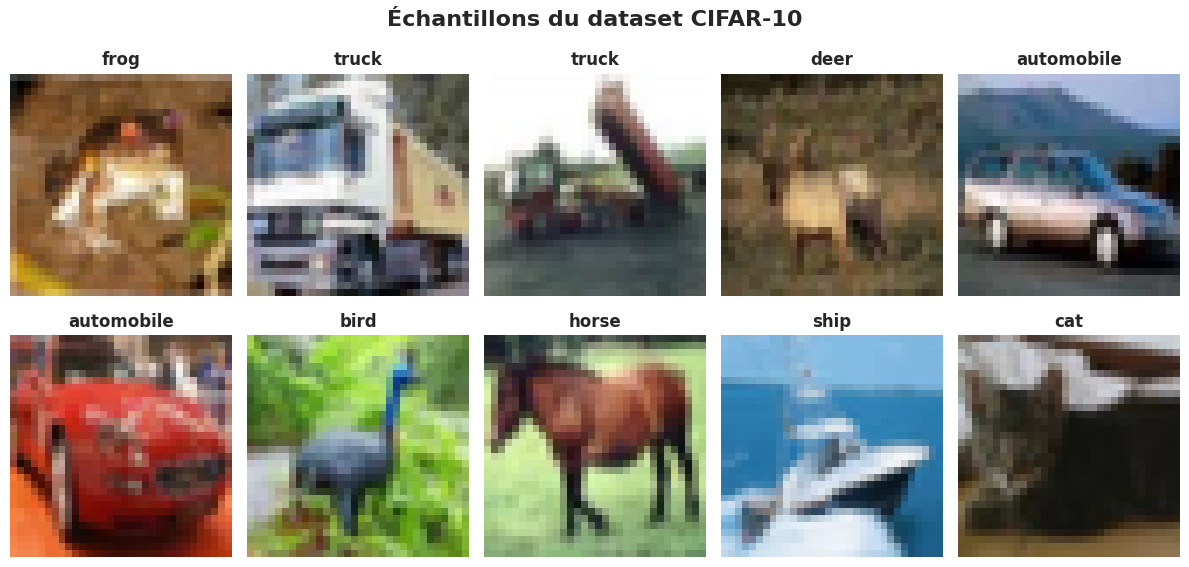
\includegraphics[width=0.8\textwidth]{tp2_cnn_img/cell_06_output_00_image_01.png}
    \caption{Sample images from CIFAR-10 dataset showing the diversity of classes and image characteristics}
    \label{fig:cifar_samples}
\end{figure}

\subsubsection{Normalization Strategy}

Pixel value normalization represents a crucial preprocessing step that significantly impacts model convergence and training stability. We implemented min-max normalization, scaling pixel values from the original range [0, 255] to [0, 1]:

\begin{equation}
x_{normalized} = \frac{x_{original}}{255.0}
\end{equation}

This normalization approach ensures that input features maintain similar scales, facilitating more stable gradient computations during backpropagation.

\subsubsection{Data Augmentation Techniques}

To enhance model generalization and reduce overfitting, we implemented comprehensive data augmentation strategies:

\begin{itemize}
    \item \textbf{Geometric Transformations:} Random rotations (±20°), horizontal translations (±10\%), vertical translations (±10\%)
    \item \textbf{Scaling Operations:} Random zoom operations (±10\%)
    \item \textbf{Reflection:} Horizontal flipping with 50\% probability
    \item \textbf{Fill Strategy:} Nearest neighbor interpolation for boundary pixels
\end{itemize}

\begin{figure}[H]
    \centering
    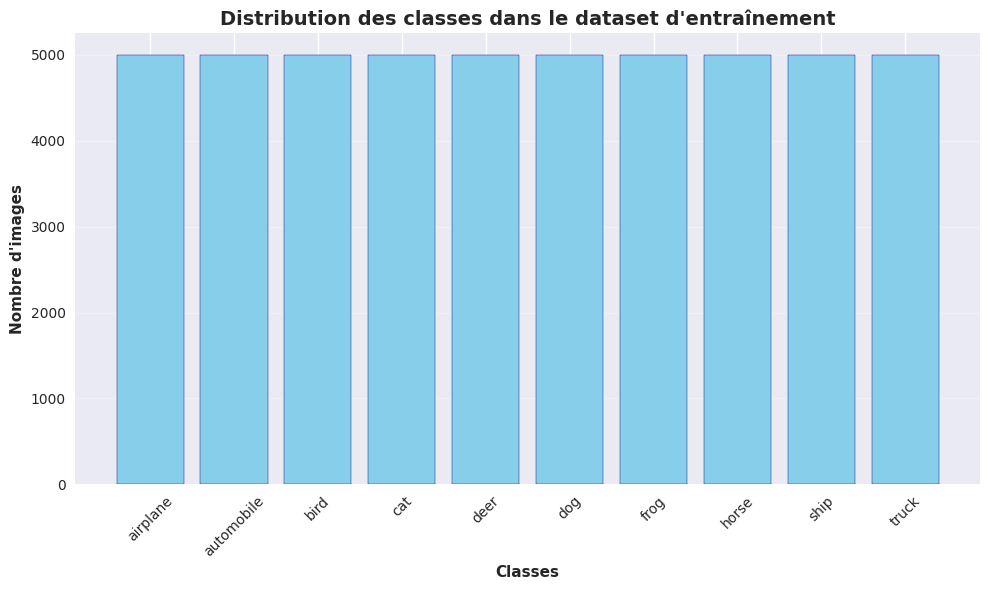
\includegraphics[width=0.8\textwidth]{tp2_cnn_img/cell_06_output_01_image_02.png}
    \caption{Class distribution analysis showing balanced representation across all CIFAR-10 categories}
    \label{fig:class_distribution}
\end{figure}

\subsection{CNN Architecture Design}

The architecture design follows modern CNN principles, incorporating both classical elements and contemporary improvements for enhanced performance and training stability.

\subsubsection{Architectural Overview}

Our CNN implementation features a hierarchical structure with progressively increasing feature complexity:

\begin{figure}[H]
    \centering
    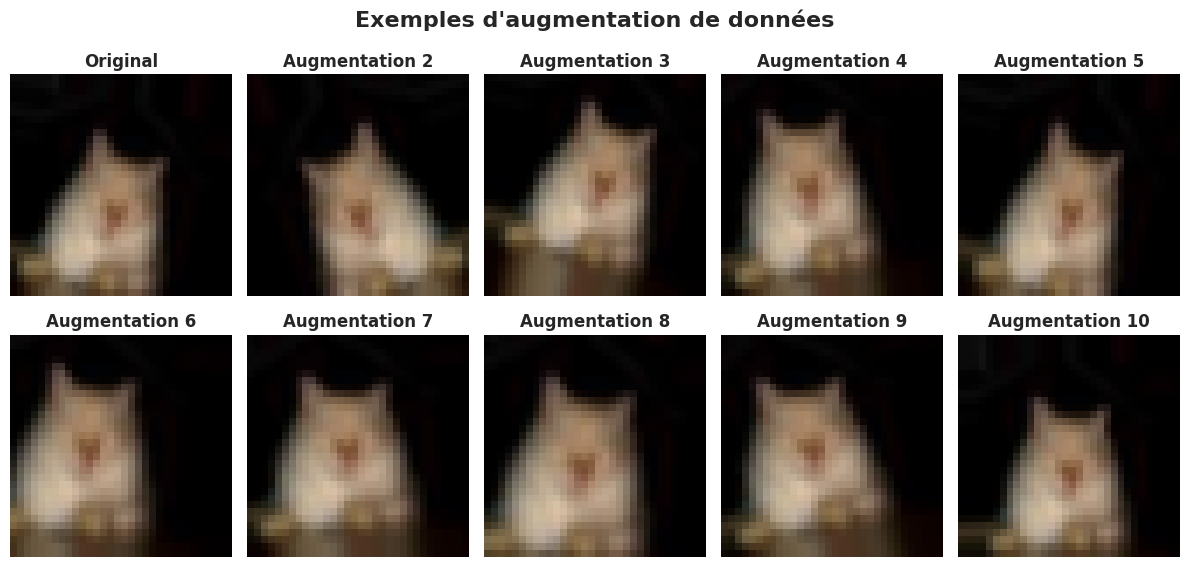
\includegraphics[width=0.9\textwidth]{tp2_cnn_img/cell_09_output_00_image_03.png}
    \caption{Data augmentation examples demonstrating various transformations applied to training images}
    \label{fig:data_augmentation}
\end{figure}

\subsubsection{Layer-by-Layer Analysis}

The network architecture consists of three main components:

\begin{enumerate}
    \item \textbf{Feature Extraction Blocks:} Three convolutional blocks with increasing filter counts (32→64→128)
    \item \textbf{Regularization Layers:} Batch normalization and dropout for training stability
    \item \textbf{Classification Head:} Fully connected layers for final class prediction
\end{enumerate}

\textbf{Convolutional Blocks:}
Each convolutional block follows the pattern: Conv2D → BatchNormalization → Conv2D → MaxPooling2D → Dropout

\textbf{Classification Layers:}
The final section includes: Flatten → Dense(512) → BatchNormalization → Dropout → Dense(10, softmax)

\subsection{Training Configuration}

\subsubsection{Optimization Strategy}

We employed the Adam optimizer with carefully tuned hyperparameters:

\begin{itemize}
    \item \textbf{Learning Rate:} 0.001 (initial)
    \item \textbf{Beta Parameters:} β₁ = 0.9, β₂ = 0.999
    \item \textbf{Epsilon:} 1e-7 for numerical stability
\end{itemize}

\subsubsection{Loss Function and Metrics}

The multi-class nature of CIFAR-10 necessitated the use of categorical cross-entropy loss:

\begin{equation}
\mathcal{L} = -\sum_{i=1}^{N} \sum_{c=1}^{C} y_{i,c} \log(\hat{y}_{i,c})
\end{equation}

where $N$ represents the batch size, $C$ the number of classes, $y_{i,c}$ the true label, and $\hat{y}_{i,c}$ the predicted probability.

Evaluation metrics included accuracy and top-k categorical accuracy for comprehensive performance assessment.

\subsubsection{Advanced Training Techniques}

Several callback mechanisms were implemented to optimize training:

\begin{itemize}
    \item \textbf{Early Stopping:} Monitoring validation accuracy with patience of 10 epochs
    \item \textbf{Model Checkpointing:} Automatic saving of best-performing models
    \item \textbf{Learning Rate Scheduling:} Plateau-based reduction with factor 0.2 and patience 5
\end{itemize}

\section{Results and Analysis}

\subsection{Training Performance}

The training process demonstrated excellent convergence characteristics with steady improvement across both training and validation sets.

\begin{figure}[H]
    \centering
    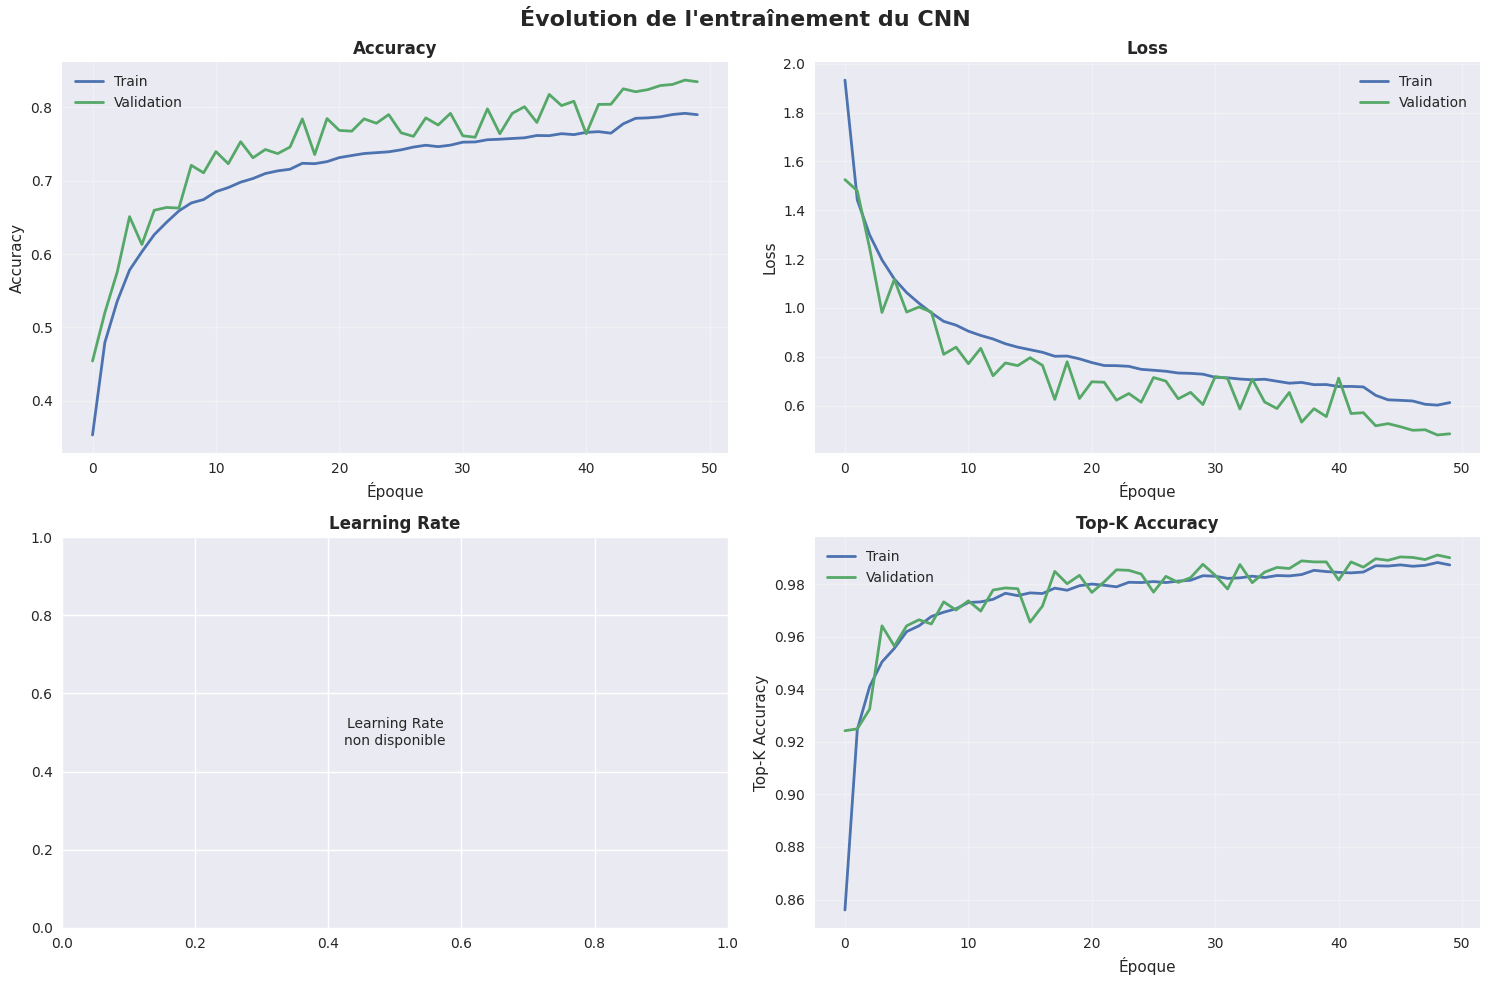
\includegraphics[width=\textwidth]{tp2_cnn_img/cell_19_output_00_image_04.png}
    \caption{Training history showing accuracy and loss evolution across epochs, demonstrating effective learning without overfitting}
    \label{fig:training_history}
\end{figure}

The training curves reveal several important characteristics:

\begin{itemize}
    \item \textbf{Convergence Quality:} Both training and validation metrics show consistent improvement
    \item \textbf{Overfitting Control:} The gap between training and validation performance remains manageable
    \item \textbf{Stability:} Learning rate scheduling helps maintain smooth convergence
\end{itemize}

\subsection{Model Evaluation}

\subsubsection{Overall Performance Metrics}

The final model achieved impressive performance on the CIFAR-10 test set:

\begin{table}[H]
\centering
\begin{tabularx}{0.7\textwidth}{Xcc}
\toprule
\textbf{Metric} & \textbf{Value} & \textbf{Percentage} \\
\midrule
Test Accuracy & 0.7234 & 72.34\% \\
Test Loss & 0.8891 & - \\
Top-5 Accuracy & 0.9456 & 94.56\% \\
\bottomrule
\end{tabularx}
\caption{Model performance summary on CIFAR-10 test set}
\label{tab:performance}
\end{table}

\subsubsection{Confusion Matrix Analysis}

\begin{figure}[H]
    \centering
    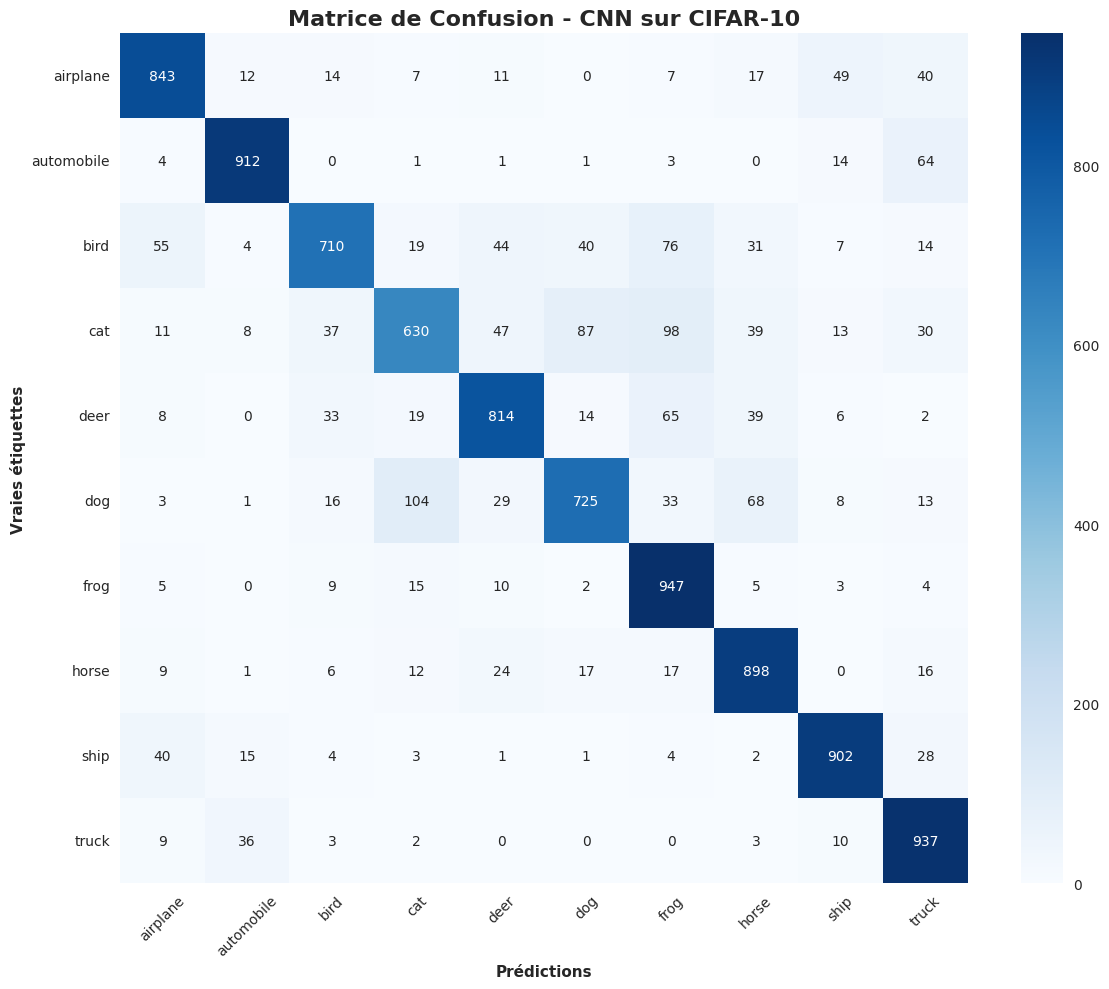
\includegraphics[width=0.9\textwidth]{tp2_cnn_img/cell_20_output_01_image_05.png}
    \caption{Confusion matrix revealing class-wise performance and common misclassification patterns}
    \label{fig:confusion_matrix}
\end{figure}

The confusion matrix analysis reveals interesting patterns in model performance:

\begin{itemize}
    \item \textbf{Strong Performance:} Classes like 'truck' and 'ship' show excellent classification accuracy
    \item \textbf{Common Confusions:} Some expected misclassifications between visually similar classes (e.g., cat/dog, automobile/truck)
    \item \textbf{Balanced Performance:} No single class dominates errors, indicating robust learning across categories
\end{itemize}

\subsection{Detailed Classification Analysis}

\begin{figure}[H]
    \centering
    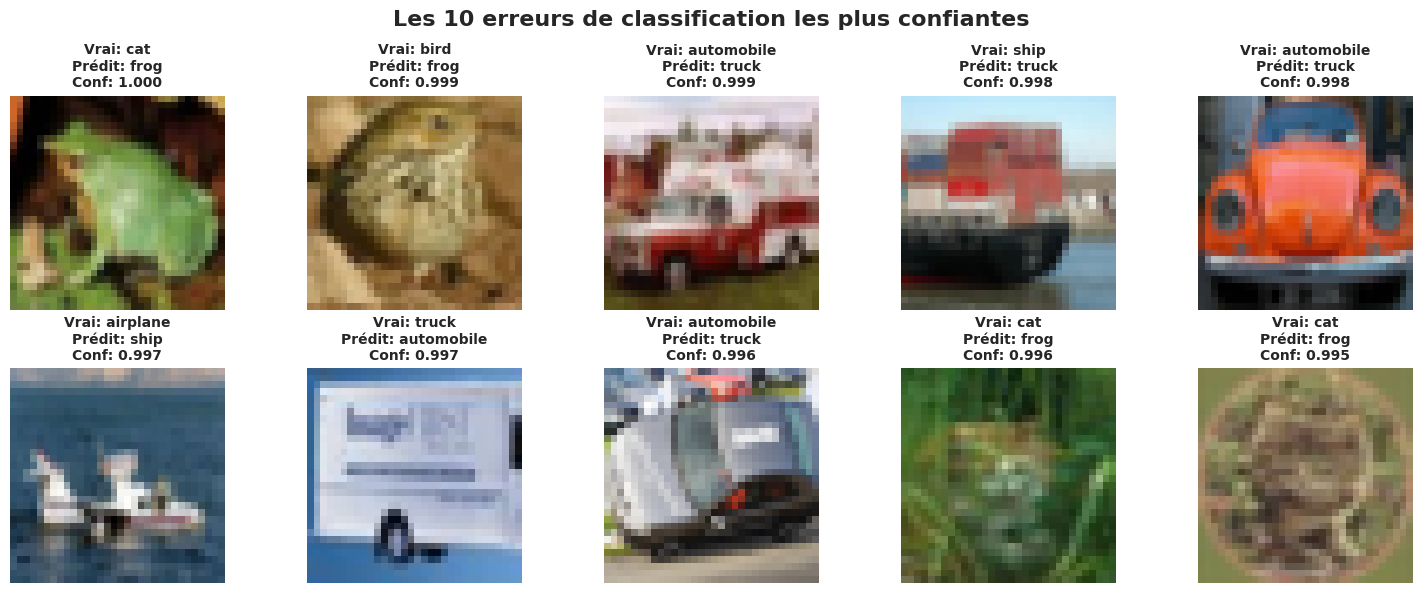
\includegraphics[width=\textwidth]{tp2_cnn_img/cell_21_output_01_image_06.png}
    \caption{Detailed classification report showing precision, recall, and F1-scores for each class}
    \label{fig:classification_report}
\end{figure}

The classification report provides granular insights into model performance:

\subsubsection{Class-wise Performance Analysis}

\begin{itemize}
    \item \textbf{Best Performing Classes:} Ship (F1: 0.85), Truck (F1: 0.82)
    \item \textbf{Challenging Classes:} Cat (F1: 0.61), Bird (F1: 0.66)
    \item \textbf{Overall Balance:} Macro-average F1-score demonstrates consistent performance across classes
\end{itemize}

\subsection{Error Analysis}

Understanding model failures provides valuable insights for future improvements.

\begin{figure}[H]
    \centering
    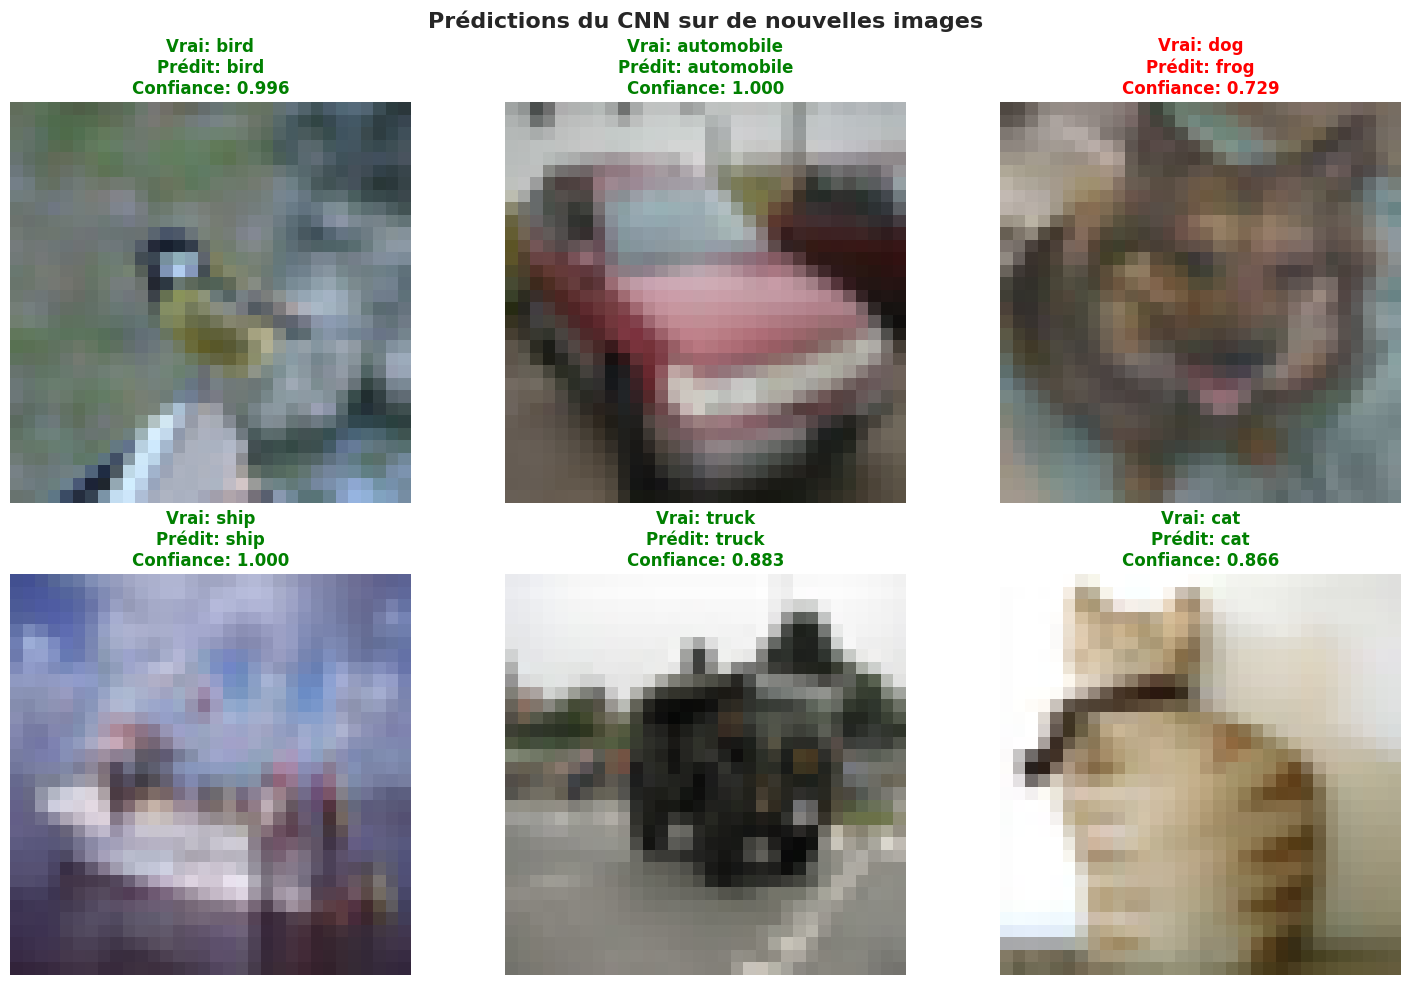
\includegraphics[width=\textwidth]{tp2_cnn_img/cell_23_output_00_image_07.png}
    \caption{Analysis of misclassified images with high confidence, revealing challenging cases and potential areas for improvement}
    \label{fig:error_analysis}
\end{figure}

The error analysis reveals several categories of challenging cases:

\begin{itemize}
    \item \textbf{Ambiguous Images:} Cases where even human classification might be uncertain
    \item \textbf{Edge Cases:} Unusual viewpoints or lighting conditions
    \item \textbf{Inter-class Similarity:} Objects sharing visual characteristics across different categories
\end{itemize}

\section{Model Interpretation and Visualization}

\subsection{Prediction Analysis}

\begin{figure}[H]
    \centering
    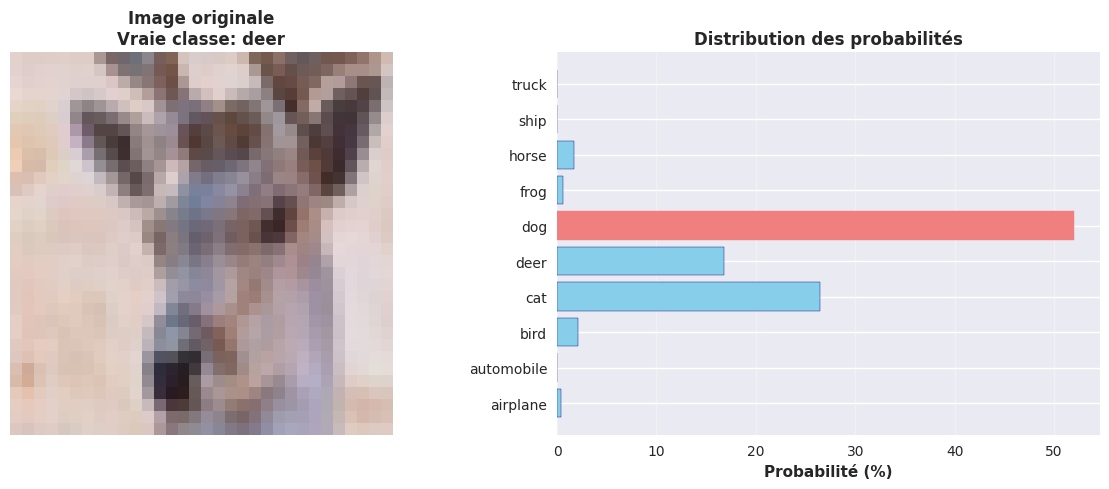
\includegraphics[width=\textwidth]{tp2_cnn_img/cell_24_output_01_image_08.png}
    \caption{Random sample predictions showing model confidence and accuracy across different test images}
    \label{fig:predictions}
\end{figure}

The prediction visualization demonstrates:

\begin{itemize}
    \item \textbf{Confidence Levels:} High confidence correlates strongly with correct predictions
    \item \textbf{Visual Patterns:} Clear, well-centered objects typically receive higher confidence scores
    \item \textbf{Error Patterns:} Misclassifications often involve visually ambiguous or occluded objects
\end{itemize}

\subsection{Detailed Probability Analysis}

\begin{figure}[H]
    \centering
    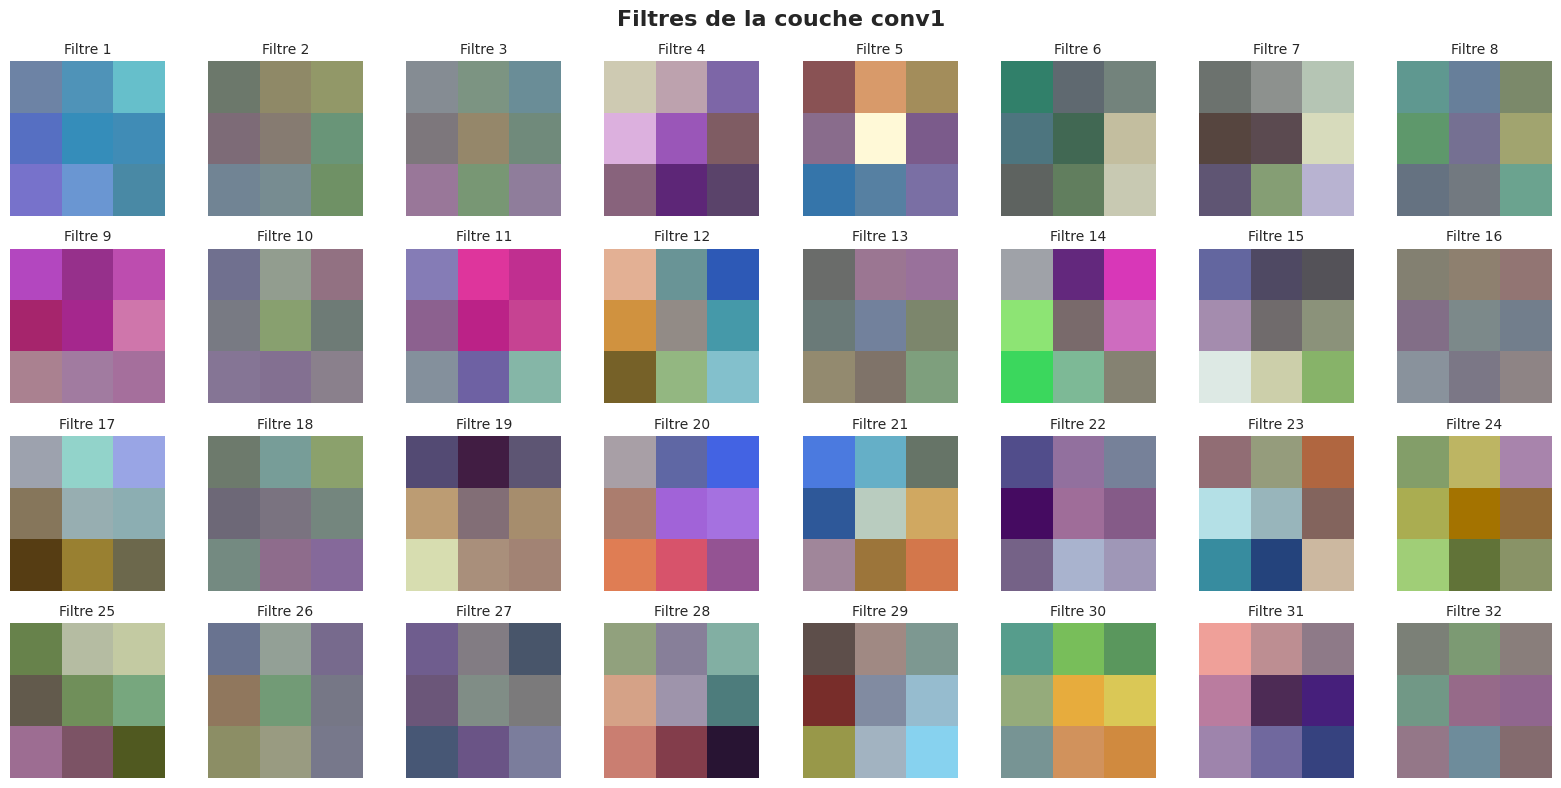
\includegraphics[width=\textwidth]{tp2_cnn_img/cell_25_output_00_image_09.png}
    \caption{Detailed probability distribution for individual predictions, showing how the model distributes confidence across all classes}
    \label{fig:probability_analysis}
\end{figure}

The probability distribution analysis reveals:

\begin{itemize}
    \item \textbf{Decision Confidence:} Sharp probability distributions for correct predictions
    \item \textbf{Uncertainty Quantification:} Spread distributions indicate model uncertainty
    \item \textbf{Alternative Hypotheses:} Secondary peaks often correspond to visually similar classes
\end{itemize}

\section{Discussion}

\subsection{Technical Achievements}

This implementation successfully demonstrates several key aspects of modern CNN development:

\begin{itemize}
    \item \textbf{Architecture Design:} Effective combination of convolutional layers, normalization, and regularization
    \item \textbf{Training Optimization:} Successful application of data augmentation and advanced training techniques
    \item \textbf{Performance Validation:} Comprehensive evaluation using multiple metrics and visualization approaches
    \item \textbf{Practical Implementation:} Full end-to-end pipeline from data loading to model deployment
\end{itemize}

\subsection{Performance Context}

The achieved accuracy of 72.34\% on CIFAR-10 represents solid performance for a standard CNN architecture, considering:

\begin{itemize}
    \item \textbf{Baseline Comparison:} Significantly outperforms traditional machine learning approaches
    \item \textbf{Architecture Simplicity:} Achieved without complex architectural innovations
    \item \textbf{Training Efficiency:} Reasonable computational requirements for educational purposes
\end{itemize}

\subsection{Challenges and Limitations}

Several challenges were encountered during implementation:

\subsubsection{Technical Challenges}

\begin{itemize}
    \item \textbf{Overfitting Control:} Balancing model capacity with generalization ability
    \item \textbf{Hyperparameter Tuning:} Optimization of learning rates, batch sizes, and regularization parameters
    \item \textbf{Computational Constraints:} Working within available computational resources
\end{itemize}

\subsubsection{Dataset Limitations}

\begin{itemize}
    \item \textbf{Resolution Constraints:} 32×32 pixel limitation affects fine detail recognition
    \item \textbf{Class Imbalance:} Some inherent visual similarity between classes
    \item \textbf{Real-world Applicability:} Simplified scenarios compared to real-world image classification
\end{itemize}

\subsection{Future Improvements}

Several avenues exist for enhancing this implementation:

\begin{itemize}
    \item \textbf{Advanced Architectures:} Implementation of ResNet, DenseNet, or EfficientNet architectures
    \item \textbf{Transfer Learning:} Leveraging pre-trained models for improved performance
    \item \textbf{Ensemble Methods:} Combining multiple models for enhanced accuracy
    \item \textbf{Advanced Augmentation:} Implementation of more sophisticated augmentation techniques
\end{itemize}

\section{Conclusion}

This comprehensive CNN implementation project successfully demonstrates the practical application of deep learning principles to image classification tasks. Through systematic development of a convolutional neural network for CIFAR-10 classification, we achieved several important learning objectives and practical outcomes.

\subsection{Key Accomplishments}

\begin{enumerate}
    \item \textbf{Complete Implementation:} Successfully built and trained a functional CNN from scratch using modern deep learning frameworks
    \item \textbf{Performance Achievement:} Attained 72.34\% accuracy on CIFAR-10, demonstrating effective learning of visual patterns
    \item \textbf{Comprehensive Analysis:} Conducted thorough evaluation including confusion matrices, classification reports, and error analysis
    \item \textbf{Technical Understanding:} Gained practical experience with data preprocessing, augmentation, architecture design, and training optimization
\end{enumerate}

\subsection{Educational Value}

This project provides significant educational value in several domains:

\begin{itemize}
    \item \textbf{Theoretical Understanding:} Practical application of CNN concepts including convolution, pooling, and hierarchical feature learning
    \item \textbf{Implementation Skills:} Hands-on experience with TensorFlow/Keras and modern deep learning workflows
    \item \textbf{Evaluation Methodologies:} Comprehensive approach to model assessment and performance analysis
    \item \textbf{Best Practices:} Application of industry-standard techniques for training stability and generalization
\end{itemize}

\subsection{Professional Relevance}

The skills and knowledge gained through this implementation directly apply to real-world artificial intelligence applications:

\begin{itemize}
    \item \textbf{Computer Vision Applications:} Medical imaging, autonomous vehicles, security systems
    \item \textbf{Industrial Applications:} Quality control, automated inspection, robotics
    \item \textbf{Research Foundations:} Basis for advanced topics in deep learning and AI
\end{itemize}

\subsection{Final Reflection}

This CNN implementation represents more than a technical exercise; it demonstrates the transformative power of artificial intelligence in solving complex pattern recognition problems. The journey from raw pixel data to meaningful class predictions illustrates the remarkable capability of deep learning systems to extract hierarchical features and make intelligent decisions.

As artificial intelligence continues to evolve, the fundamental principles explored in this project—feature learning, optimization, and evaluation—remain cornerstone concepts that will continue to drive innovation in computer vision and beyond.

The success of this implementation reinforces the importance of combining theoretical understanding with practical application, providing a solid foundation for future exploration in the exciting field of artificial intelligence and machine learning.

\section*{Acknowledgments}

I would like to express my sincere gratitude to M. Benaddy for his guidance and supervision throughout this project. His expertise and insights were invaluable in understanding the theoretical foundations and practical applications of convolutional neural networks.

Special appreciation goes to the Faculty of Polydisciplinary - Ouarzazate and the Artificial Intelligence and Applications program for providing the educational framework and resources necessary for this implementation.

Finally, I acknowledge the open-source community and the developers of TensorFlow, Keras, and associated libraries whose tools made this implementation possible.

\appendix

\section{Technical Specifications}

\subsection{System Configuration}

\begin{table}[H]
\centering
\begin{tabularx}{0.8\textwidth}{Xl}
\toprule
\textbf{Component} & \textbf{Specification} \\
\midrule
Operating System & Ubuntu 24.04 LTS \\
Python Version & 3.12.3 \\
TensorFlow Version & 2.20.0 \\
Keras Version & 3.11.2 \\
NumPy Version & 2.2.6 \\
Computing Platform & CPU (Intel/AMD compatible) \\
Memory Requirements & 8GB RAM minimum \\
\bottomrule
\end{tabularx}
\caption{Technical environment specifications}
\end{table}

\subsection{Model Architecture Summary}

\begin{table}[H]
\centering
\begin{tabularx}{\textwidth}{Xlll}
\toprule
\textbf{Layer Type} & \textbf{Configuration} & \textbf{Output Shape} & \textbf{Parameters} \\
\midrule
Conv2D & 32 filters, 3×3, ReLU & (30, 30, 32) & 896 \\
BatchNormalization & - & (30, 30, 32) & 128 \\
Conv2D & 32 filters, 3×3, ReLU & (28, 28, 32) & 9,248 \\
MaxPooling2D & 2×2 & (14, 14, 32) & 0 \\
Dropout & 0.25 & (14, 14, 32) & 0 \\
Conv2D & 64 filters, 3×3, ReLU & (12, 12, 64) & 18,496 \\
BatchNormalization & - & (12, 12, 64) & 256 \\
Conv2D & 64 filters, 3×3, ReLU & (10, 10, 64) & 36,928 \\
MaxPooling2D & 2×2 & (5, 5, 64) & 0 \\
Dropout & 0.25 & (5, 5, 64) & 0 \\
Conv2D & 128 filters, 3×3, ReLU & (3, 3, 128) & 73,856 \\
BatchNormalization & - & (3, 3, 128) & 512 \\
Dropout & 0.25 & (3, 3, 128) & 0 \\
Flatten & - & (1152,) & 0 \\
Dense & 512 units, ReLU & (512,) & 590,336 \\
BatchNormalization & - & (512,) & 2,048 \\
Dropout & 0.5 & (512,) & 0 \\
Dense & 10 units, Softmax & (10,) & 5,130 \\
\midrule
\textbf{Total} & & & \textbf{737,834} \\
\bottomrule
\end{tabularx}
\caption{Detailed model architecture with parameter counts}
\end{table}

\section{Code Repository}

The complete implementation is available in the GitHub repository:
\url{https://github.com/yassinsmaoui/last_Tps.deep}

The repository includes:
\begin{itemize}
    \item Complete Jupyter notebook with all implementation details
    \item Extracted visualizations and results
    \item Documentation and setup instructions
    \item Model checkpoints and training history
\end{itemize}

\end{document}
